\documentclass[border=12pt]{standalone}
\def\pgfsysdriver{pgfsys-dvisvgm.def}
\usepackage[dvisvgm]{xcolor}
\usepackage{xeCJK}
\setCJKmainfont{HaranoAjiGothic-Regular.otf}[BoldFont=HaranoAjiGothic-Bold.otf]
\setCJKsansfont{HaranoAjiGothic-Regular.otf}[BoldFont=HaranoAjiGothic-Bold.otf]
\usepackage{amsmath,amssymb,tikz,lmodern}
\usetikzlibrary{arrows.meta,positioning,calc,fit,backgrounds}
\renewcommand{\familydefault}{\sfdefault}
\definecolor{ink}{HTML}{25322F}
\definecolor{green}{HTML}{246657}
\definecolor{tint}{HTML}{EEF4F0}
\definecolor{soft}{HTML}{C6D2CC}
\definecolor{muted}{HTML}{52615B}
\newif\ifJapanese
\newcommand{\Tx}[2]{\ifJapanese #1\else #2\fi}
\newcommand{\Eff}{\overline{\operatorname{Eff}}}
\newcommand{\heading}[3]{{\color{green}\bfseries #1\quad\Tx{#2}{#3}}\\[5pt]}
% A white rectangle makes the complete citation label clickable, including spaces.
\newcommand{\refurl}[2]{\special{dvisvgm:raw <a xlink:href="#1" target="_blank" rel="noopener noreferrer">}{\setlength{\fboxsep}{0pt}\colorbox{white}{\color{green}\underline{\strut #2}}}\special{dvisvgm:raw </a>}}
\newcommand{\refedge}[3]{\refurl{\csname source#1\endcsname\string##page=#2}{#3}}
\newcommand{\SF}[2]{\refedge{sf}{#1}{#2}}
% GitHub's file preview does not support PDF page fragments.
\newcommand{\LA}[2]{\refurl{\sourcela}{#2}}
\newcommand{\Sch}[2]{\refedge{sch}{#1}{#2}}
\newcommand{\PS}[2]{\refedge{ps}{#1}{#2}}
\tikzset{
 card/.style={draw=soft,fill=white,rounded corners=2pt,align=left,text=ink,font=\fontsize{10.5}{14}\selectfont,inner xsep=12pt,inner ysep=10pt,text width=14.4cm},
 half/.style={card,text width=6.45cm,minimum height=2.05cm},
 result/.style={card,draw=green,fill=tint,line width=.9pt},
 reason/.style={align=left,text=muted,font=\fontsize{9}{12}\selectfont,inner sep=0pt,text width=12.7cm},
 branchreason/.style={reason,text width=5.95cm},
 edge/.style={-{Stealth[length=2.4mm]},draw=green,line width=1pt},
 wire/.style={draw=green,line width=1pt},
}
% Keep the arrow in a dedicated left gutter; explanations never cover it.
\newcommand{\flow}[3]{
 \coordinate (#2-from) at ($(#1.south)+(-6.9,0)$);
 \coordinate (#2-to) at ($(#2.north)+(-6.9,0)$);
 \draw[edge] (#2-from)--(#2-to);
 \node[reason,anchor=west] (#2-reason) at ($(#2-from)!.5!(#2-to)+(.55,0)$) {#3};
}
\newcommand{\Cite}[2]{\refurl{\csname source#1\endcsname}{#2}}

\Japanesefalse
\newcommand{\sourceslc}{https://github.com/openai/math/blob/adc7f1241b42e322a6451854ab7e4b4c146bf78a/preprints/Uniform-indices-for-semi-log-canonical-log-Calabi-Yau-pairs-October-5-2026/uniform-slc-index.pdf}
\newcommand{\sourceui}{https://github.com/openai/math/blob/adc7f1241b42e322a6451854ab7e4b4c146bf78a/preprints/Uniform-Pluricanonical-Iitaka-Fibrations-October-3-2026/paper.pdf}
\newcommand{\sourcela}{https://github.com/openai/math/blob/adc7f1241b42e322a6451854ab7e4b4c146bf78a/preprints/Log-abundance-in-characteristic-zero-September-24-2026/paper.pdf}
\newcommand{\sourceuli}{https://github.com/openai/math/blob/adc7f1241b42e322a6451854ab7e4b4c146bf78a/preprints/Uniform-log-Iitaka-fibrations-and-bounded-moduli-denominators-October-4-2026/uniform-log-iitaka.pdf}
\newcommand{\sourcek}{https://arxiv.org/pdf/1107.2863v3}
\newcommand{\sourcehj}{https://arxiv.org/pdf/2204.04946v2}
\newcommand{\sourcejl}{https://arxiv.org/pdf/2002.11928}
\begin{document}
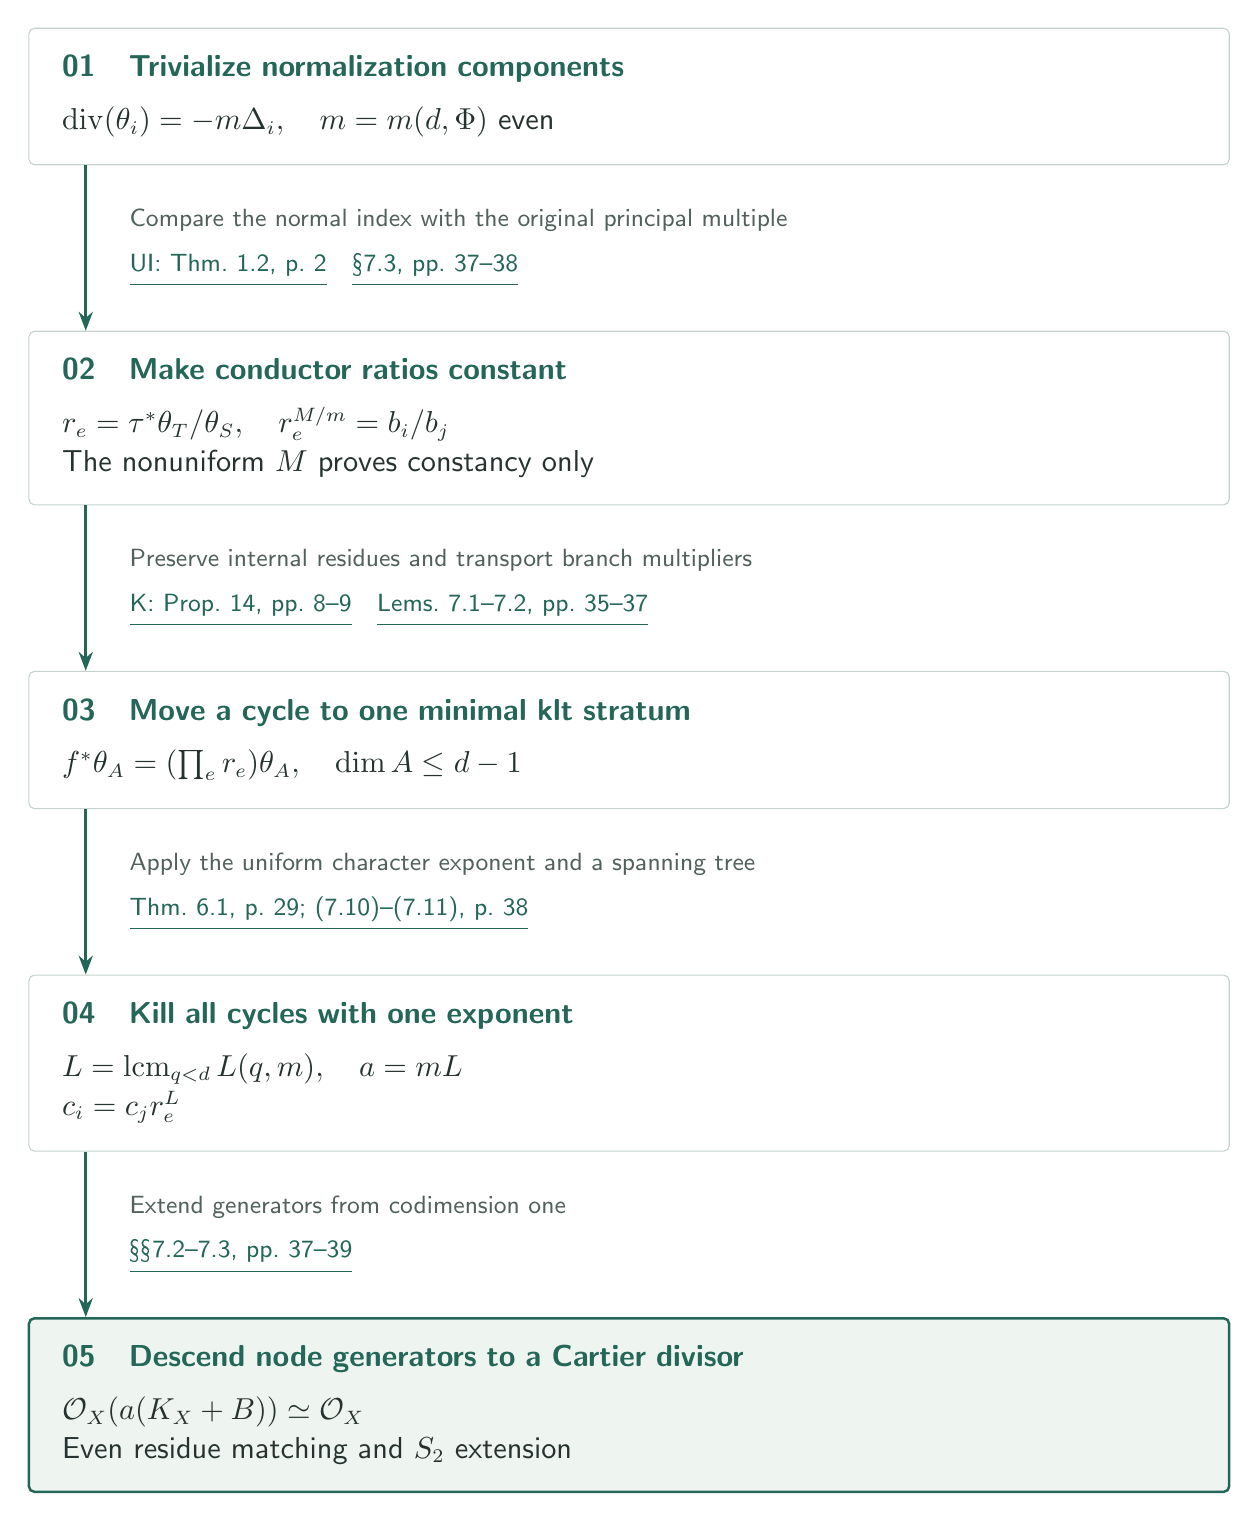
\begin{tikzpicture}
\node[card] (n0) {\heading{01}{正規化の各成分を自明化}{Trivialize normalization components}\Tx{$\operatorname{div}(\theta_i)=-m\Delta_i,\quad m=m(d,\Phi)\ \text{even}$}{$\operatorname{div}(\theta_i)=-m\Delta_i,\quad m=m(d,\Phi)\ \text{even}$}};
\node[card,below=2.1cm of n0] (n1) {\heading{02}{conductorの比を定数にする}{Make conductor ratios constant}\Tx{$r_e=\tau^*\theta_T/\theta_S,\quad r_e^{M/m}=b_i/b_j$\\非一様な $M$ は定数性のみに使う}{$r_e=\tau^*\theta_T/\theta_S,\quad r_e^{M/m}=b_i/b_j$\\The nonuniform $M$ proves constancy only}};
\flow{n0}{n1}{\Tx{normal lc指数と元の主因子を比較}{Compare the normal index with the original principal multiple}\\[4pt]\Cite{ui}{UI: Thm.\ 1.2, p.\ 2}\quad \Cite{slc}{\S7.3, pp.\ 37--38}}
\node[card,below=2.1cm of n1] (n2) {\heading{03}{閉路を最小klt stratumへ移す}{Move a cycle to one minimal klt stratum}\Tx{$f^*\theta_A=(\prod_e r_e)\theta_A,\quad \dim A\leq d-1$}{$f^*\theta_A=(\prod_e r_e)\theta_A,\quad \dim A\leq d-1$}};
\flow{n1}{n2}{\Tx{内部の留数保存と枝を渡る同倍率写像}{Preserve internal residues and transport branch multipliers}\\[4pt]\Cite{k}{K: Prop.\ 14, pp.\ 8--9}\quad \Cite{slc}{Lems.\ 7.1--7.2, pp.\ 35--37}}
\node[card,below=2.1cm of n2] (n3) {\heading{04}{全閉路を同じ冪で消す}{Kill all cycles with one exponent}\Tx{$L=\operatorname{lcm}_{q<d}L(q,m),\quad a=mL$\\$c_i=c_jr_e^L$}{$L=\operatorname{lcm}_{q<d}L(q,m),\quad a=mL$\\$c_i=c_jr_e^L$}};
\flow{n2}{n3}{\Tx{klt指標の一様指数を全域木に適用}{Apply the uniform character exponent and a spanning tree}\\[4pt]\Cite{slc}{Thm.\ 6.1, p.\ 29; (7.10)--(7.11), p.\ 38}}
\node[result,below=2.1cm of n3] (n4) {\heading{05}{node上の生成元からCartier降下}{Descend node generators to a Cartier divisor}\Tx{$\mathcal O_X(a(K_X+B))\simeq\mathcal O_X$\\偶数次数の留数照合と $S_2$ 延長}{$\mathcal O_X(a(K_X+B))\simeq\mathcal O_X$\\Even residue matching and $S_2$ extension}};
\flow{n3}{n4}{\Tx{codimension oneの生成元を延長}{Extend generators from codimension one}\\[4pt]\Cite{slc}{\S\S7.2--7.3, pp.\ 37--39}}
\end{tikzpicture}
\end{document}
